\chapter{Deep Learning}\label{deepNets}
\chapterauthor{Jeff Yoshimi}

% Glossary items for bold faced items in this section.
% Replace deepNets with deepLearning and cohere with back references
% Lots of weight layers and node layers. Cohere.
% Remember our notation, it gets even crazier!
% Filter weights?

%So both the node and weight layers of a deep feed-forward network are different from the standard feed-forward networks we considered in other chapters. The convolutional weight layers are these floating filters that are scanned over an input layer, and the node layers are tensors which are often arrays of matrices. But note that deep networks don't \emph{only} use these fancy layers. 

% Other topics: pooling, strides, or padding (mention in footnote)
% Discuss engineering, connectionism, CCN, and comp neuro. Maybe make that a final section
% Discuss deep fakes and GANs

The idea of re-mapping an input space to a hidden unit space in order to solve classification and regression problems is what drew neural networks out of its first ``dark age'' and back into the limelight, giving rise to explosion of interest in engineering and connectionism in the 1980s and 1990s (chapter \extref{ch_history}). These internal representations allowed networks to  solve previously unsolvable problems, as we've seen, but in addition, they developed psychologically realistic internal representations, as we will see. However, recall that a second  winter lay in wait, as machine learning models took over in the late 1990s and 2000s and as backprop  ran up against various limitations. This second winter was overcome starting in the 2010s with various technological and conceptual advances, including availability of big data, graphical  processing units for  fast parallel computation, and slight changes in network architecture and structure--like the Relu activation function discussed in chapter \extref{ch_act_functions}. These advances made it possible to use the same supervised learning methods discussed throughout this chapter to train ``deep networks'', feed-forward networks with many layers to solve problems that could not be solved before.\footnote{This history is well told by Kurenkov in section 3 of \url{https://www.skynettoday.com/overviews/neural-net-history}. As he summarizes, ``Deep Learning = Lots of training data + Parallel Computation + Scalable, smart algorithms.''} 
% Summarize main history in footnote. Vanishing gradients. Relu. Automatic differentiation. Availability of big data. GPU.
% Generalized techniques for effectively performing gradient descent on many kinds of architectures were developed. This is called automatic differentiation. Basically very complex calculus. These also made it possible to parallelize much of this work. A standardized language for discussing these networks also emerged, via the dominance of a few programs: keras, tensorflow, etc. 

This resurgence of interest  in neural networks was--like the first one--a boon to both engineering neural networks and to connectionism, as well as neuroscience. These many-layered trained networks could solve new problems, that earlier networks could not solve, producing huge improvements in image recognition, speech recognition, language translation, and other areas. They did this by creating hierarchies of representations, corresponding  to increasingly complex features of an input image. As we saw in chapter \extref{ch_neuro} (see figure \extref{deepLearning_Vision}) when such networks are trained to recognize images they develop internal representation that are extremely similar to those developed by the human visual  system.
% Citation and sources and a better list of what these advances were

The topic of deep networks and deep learning are quite involved (this is a small, preliminary chapter on the important topic; it will be expanded in the future). Here we will simply describe some of the main concepts.

\section{Convolutional Layers}

% Glossary and back cohere with linear algebra
The key idea is to use a special type of weight layer called a ``convolutional layer'' to efficiently learn to recognize features in a previous layer.  A standard weight layer, like what we've been working with, is sometimes referred to as a dense layer by contrast (a third kind of layer is a sparse layer, but we won't discuss that). 

To understand how a convolutional  layer works we can begin with the concept of a \textbf{filter} or \textbf{kernel}, which is a  matrix of values that is ``passed'' or ``scanned'' over an input vector.\footnote{Glossary entries are not yet written for the bold-faced items in this section.}  This process of scanning the weight matrix over the input and producing a feature map is called a \textbf{convolution}. To see how this scanning works it helps to see an animation. A good one to start with is the first animated gif here: \url{https://stanford.edu/~shervine/teaching/cs-230/cheatsheet-convolutional-neural-networks}.\footnote{This link also introduces some of the concepts we are not discussing here, such strides, and padding, which are used to specify how the scanning operation of a filter works, and pooling, which combines the results of a convolutional layer into a smaller  condensed representation that is more manageable for other layers to deal with.} Note that this is totally different from the weights we have been studying throughout the book: there are no fixed connections at all. Instead it is like there is a little floating scanner that gets passed over an input layer to produce an output layer.

\begin{figure}[h]
\centering
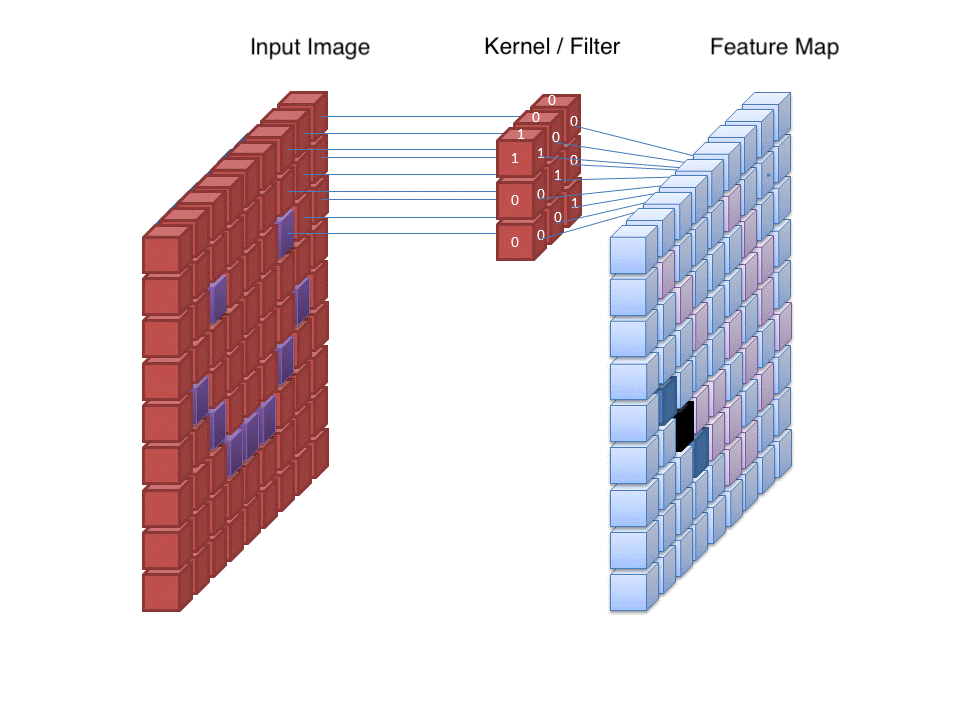
\includegraphics[width=0.5\textwidth]{images/CNN_Filter.png}
\caption[User Cecbur, \url{https://commons.wikimedia.org/wiki/File:Convolutional_Neural_Network_NeuralNetworkFilter.gif}, with labels added by Jeff Yoshimi.]{From left to right: an input image, a 3x3 convolutional filter (which detects edges with a $-45^\circ$ angle), and the resulting feature map. The filter is scanned across the image. At each stage of this scanning process, the dot product of the filtter's receptive field in the input image is computed and used to populate the feature map. This whole process is known as a convolution and a layer like this is a convolutional layer.}
\label{cnn_filter}
\end{figure}

The idea is illustrated in figure \ref{cnn_filter}. A $3 \times 3$ filter is passed over a small image, from left to right and top to bottom. At each moment during this scanning process the dot product (see chapter \extref{ch_linear_algebra}) is computed between the kernel and its ``receptive field'' in the source matrix (the part of the image the filter is on top of). That is, we simply multiply the weights times all the input activations in  the receptive field and  add them up. The result is used to populate a new layer that is called a \textbf{feature map}. In the example, the filter is an edge detector, that detects edges at a $-45^\circ$ angle, that is, edges shaped like a backslash `\textbackslash'. In the resulting feature map, notice that the highest activation is on the left side of the input image's smile, where the dot product is 2 or 3. The dot product in other parts of the image is 0 or 1. Thus the feature map shows where this kind of edge occurs in the input image.

Note that this edge detector is not programmed in. This is a neural network after all, and neural networks are trained, not programmed (section \extref{intro_comp_nn}), usually using a form of gradient descent (section \extref{sect_gradient_descent}). There is a performance advantage to these convolutional layers. All that must be trained is (in the example shown in figure \ref{cnn_filter}) $3 \times 3=9$ weights, rather than the $100 \times 100 = 10,000$ weights that would be required in a fully connected layer from the input image to the feature map. This is a huge performance gain and part of what  made it possible with deep learning to train such large networks.

% This is a bit of new idea though, so think about it. It's the same template of supervised learning. The result is not a random weight matrix mapping, but a set of filters that are used to pass over an input. FOR NEXT SECTION?



\begin{figure}[h]
\centering
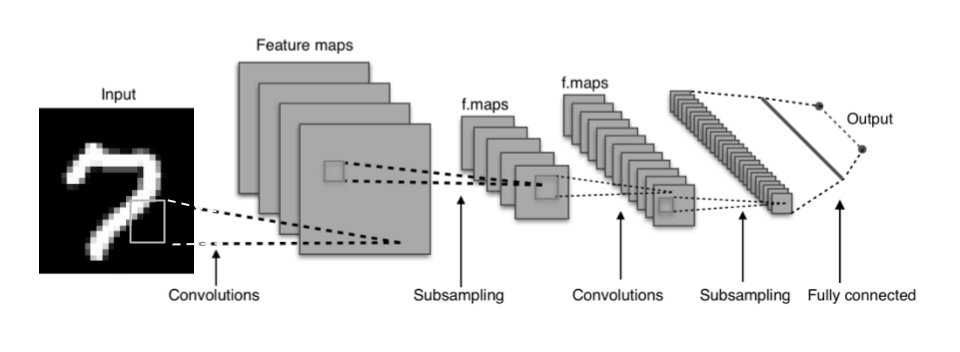
\includegraphics[scale=.45]{./images/deepNet.png}
\caption[Adapted from a creative commons image by Aphex34 at \url{https://commons.wikimedia.org/wiki/File:Typical_cnn.png} ]{A deep neural network, trained to recognize images. The convolutional layers scan over the inputs they are linked to. }
\label{deep_net2}
\end{figure}

%\begin{figure}[h]
%\centering
%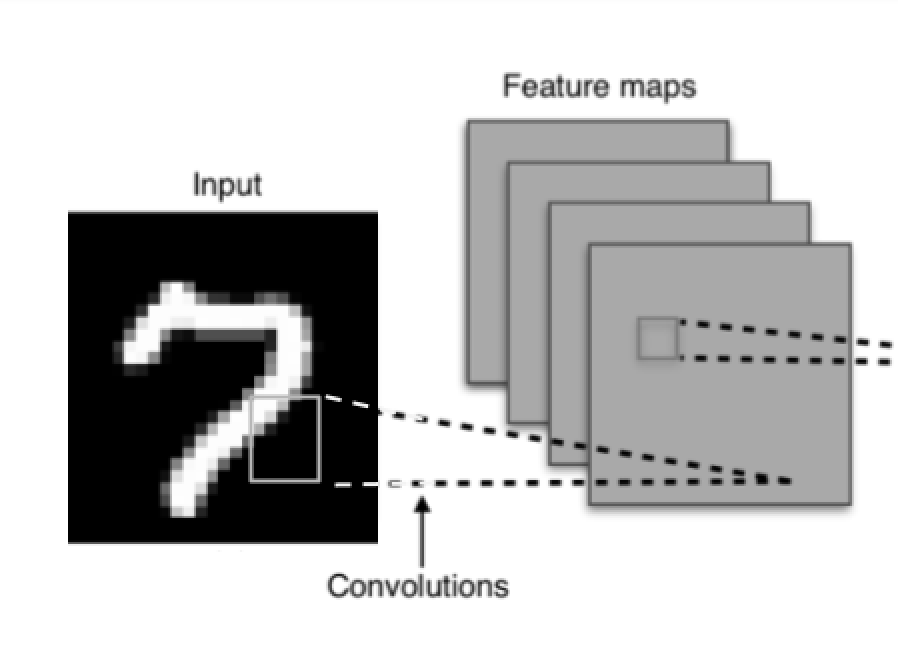
\includegraphics[scale=.4]{./images/deepNetCloseup.png}
%\caption[Closeup from a creative commons image by Aphex34 at \url{https://commons.wikimedia.org/wiki/File:Typical_cnn.png} ]{Closeup of deep neural network in chapter \extref{ch_intro} figure \extref{deep_net} showing how a set of convolutional filters like the one in \ref{cnn_filter} produce a set of feature maps. This set of feature maps is like an array of matrices, which is also known as a tensor.}
%\label{deep_net_closeup}
%\end{figure}

\section{Feature Maps and tensors}

The magic really starts to happen when we train a \emph{set of filters}, each of which produces a separate feature map.  Figure \ref{deep_net2} illustrates the idea. Note how several of the node layers say ``Feature maps'' plural, or "F.maps''. Each feature map in one of these sets is a response to a different filter, for example, edges of different orientation. This is exactly how primary visual cortex reacts to images, so this is a nice model of the brain, hence an example of computational  neuroscience. However, it is also useful to build these things for visual recognition, so it is also a good engineering example.

A few things to note here.

First, this set of feature maps is new a new kind of node layer. It is not just a  single set of nodes, but rather is itself a whole array of matrices. It's like a stack of pancake, if each pancake is a matrix.  An array of matrices is a special kind of \textbf{tensor} (a generalization of the vectors and matrices we discussed in chapter \extref{ch_linear_algebra} to more complex numerical structures), and so computations in deep networks often involve the use of tensor mathematics.\footnote{Technically numbers and vectors and matrices are also tensors. The rank of a  tensor is the number of indices it takes to specify an ``entry'' in the tensor. A number is rank 0 because it requires no indices. Recall that a vector is like a list of numbers. A vector is rank 1 because it takes one index to specify an entry in a vector. A matrix is rank 2 (it takes to numbers to specify a row and column). The tensor shown in the main text is rank 3, because it takes 3 indices: one to specify a location in the array, and then a row and column index.}  

Second, again. these networks are trained.  This is kind of remarkable to ponder. We did not tell the network we want it to learn to respond to edges. All we focus on in training a network is inputs and outputs, using a labeled data set (section \extref{sect_supervised_schema}).  In the case shown in the figure, the algorithm focuses on classifying images as numbers. So the network adjusts all the parameters (all the weight layers, including the convolutional layers and filter weights), in such a way as to reduce error. And it just so happens by this process that edge detectors are useful for this, so that's what the network learns. Edge detectors were learned by training, not programmed in.

\section{The many layers of a deep network}

In a full deep network many convolutional layers and regular ``dense'' weight layers are combined . Sometimes as many as 100 or more! This allows the network to learn to identify not just simple features like edges or curves, but also \emph{features of features}, like combinations of curves which make more complex shapes, and then combinations of these shapes. 

As can be seen in  \ref{deep_net2}, there are other kinds of relations between layers. Subsampling refers to methods where out of a part of matrix, the average is taken, or the largest value. This idea comes in various forms. The idea is to reduce the overall number of parameters over time. We will not discuss this in detail.

The final layers of a deep network are often more conventional fully-connected dense layers. The idea is to have a bunch of early layers learn these very complex features, and then to present the results to the final layers, which are basically a more conventional backprop network like the ones discussed in the last section. It's just that the inputs to these networks are particularly complex.


\section{Applications of Deep Learning}

As discussed in section \extref{deep_revolution}, deep networks and deep learning led to a revolution in neural networks beginning in the 2010s. The revolution was in engineering initially, but the history of deep networks shows that they have applications across all the domains of neural network research: engineering, computational neuroscience, and connectionism. 

They grew out of computational neuroscience models of vision in the 1970s and 1980s \cite{fukushima1982neocognitron}.  These ideas later were used to build better pattern recognition networks, an engineering application. Famous early applications included recognizing zip codes written on envelopes \cite{lecun1989backpropagation}. As deep networks became mainstream based on technical improvements (big data, GPU and hardware acceleration, better architectures and training algorithms), scientists began using them, for example, to model the response profile of neurons in the visual system (recall the discussion of figure \extref{deepLearning_Vision} in chapter \extref{ch_neuro}). 

The idea is also relevant to connectionism and computational cognitive neuroscience. You may recall from the history chapter that this idea goes  back to Oliver Selfridge and his pandemonium model, which at the time just speculated that in seeing letters a hierarchy of ``demons'' pass messages along: from edge demons to curve edges and finally to the output layer's ``B demon'' (see figure \extref{selfridge} in chapter \extref{ch_history}). These networks learn in the exact same way, but we can actually  see what their receptive fields are, and the results are sometimes strange and even disturbing.\footnote{See \url{https://distill.pub/2017/feature-visualization/} for some striking demonstrations.} 
% Work more on interpreting what is happening in that distll article, and add some material here, including pictures of the weird features. Then add some colab demos to the course.
